\subsection{Kalibrasi Sensor}

Terdapat tiga sensor utama yang digunakan dalam sistem lokalisasi dengan Kalman Filter yaitu IMU, odometri roda, dan GPS.
Setiap sensor diperlukan kalibrasi dan pengukuran nilai kovarians untuk menentukan tingkat kepercayaan Kalman Filter terhadap masing-masing sensor.

\subsubsection{Kalibrasi IMU}

Kalibrasi IMU dilakukan dengan merekam data IMU yang terpasang pada kendaraan dalam kondisi diam dan berada di permukaan yang rata selama 4 jam untuk memastikan stabilitas data dan mendapatkan karakteristik yang sesuai.
Data yang direkam kemudian dianalisis menggunakan metode Allan Variance dan mendapatkan hasil karakteristik yang ditampilkan pada Tabel~\ref{tab:allan_variance}.
Kemudian nilai kalibrasi diberikan faktor inflasi untuk memberi margin keamanan dalam estimasi.
Nilai derau akselerometer pada sumbu X dan Y digunakan sebagai dasar penentuan matriks kovarians derau proses (Q) yang merepresentasikan ketidakpastian model sistem.

\begin{table}[H]
\centering
\caption{Karakteristik derau IMU dari analisis Allan Variance (100 Hz, dengan faktor inflasi)}
\label{tab:allan_variance}
\begin{tabular}{l c c c c}
\hline
\textbf{Parameter} & \textbf{Sumbu X} & \textbf{Sumbu Y} & \textbf{Sumbu Z} & \textbf{Satuan} \\
\hline
\multicolumn{5}{c}{\textbf{Giroskop (inflasi $\times2$)}} \\
\hline
Derau Giroskop  & $1{,}279\times10^{-5}$ & $2{,}772\times10^{-5}$ & $2{,}297\times10^{-6}$ & (rad/s)$^2$ \\
Bias Giroskop   & $2{,}121\times10^{-11}$ & $4{,}097\times10^{-11}$ & $3{,}808\times10^{-12}$ & (rad/s)$^2$ \\
\hline
\multicolumn{5}{c}{\textbf{Akselerometer (inflasi $\times10$)}} \\
\hline
Derau Akselerometer     & $4{,}080\times10^{-3}$ & $1{,}988\times10^{-3}$ & $4{,}285\times10^{-3}$ & (m/s$^2$)$^2$ \\
Bias Akselerometer      & $2{,}000\times10^{-9}$ & $9{,}800\times10^{-10}$ & $4{,}500\times10^{-9}$ & (m/s$^2$)$^2$ \\
\hline
\end{tabular}
\end{table}

Data akselerasi IMU yang direkam dalam kerangka sensor harus dirotasi ke kerangka acuan lokal dunia atau \emph{Local World Aligned} (LWA) sebelum digunakan sebagai masukan Kalman Filter.
Transformasi dari kerangka sensor ke kerangka dunia merupakan langkah fundamental dalam fusi sensor multimodal, sebagaimana dijelaskan oleh \textcite{Bloesch2012StateEstimation} di mana data IMU yang diukur pada kerangka badan robot harus dirotasi ke kerangka inersia melalui matriks rotasi.
Orientasi \emph{yaw} IMU dikoreksi dengan ofset dari sudut hadap GPS yang diperoleh ketika sinyal dalam kondisi baik.

\subsubsection{Kalibrasi Odometri}

Kalibrasi odometri roda dilakukan dua tahap, yaitu kalibrasi kecepatan dan pengukuran varians odometri roda.
Kalibrasi kecepatan dilakukan dengan menggerakkan kendaraan melewati titik acuan yang berjarak 1 meter kemudian dicatat setiap kendaraan melewati titik acuan menggunakan \emph{stopwatch} yang ditunjukkan pada Gambar~\ref{fig:kalibrasi_odometri}.
Proses ini diulang sebanyak 6 kali untuk mendapatkan rata-rata waktu tempuh yang kemudian digunakan untuk menghitung kecepatan rata-rata kendaraan.

\begin{figure}[H]
    \centering
    \begin{subfigure}[b]{0.25\textwidth}
        \centering
        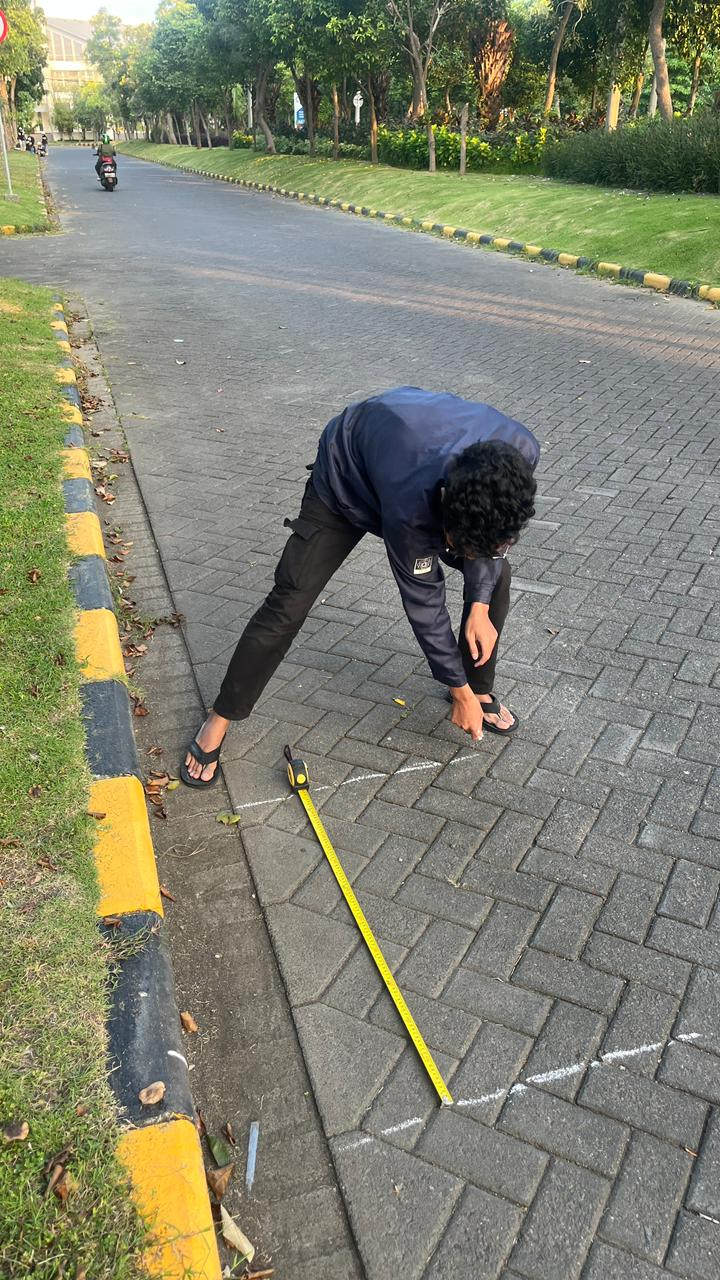
\includegraphics[width=\textwidth]{gambar/foto_kalibrasi_runtime.jpeg}
        \caption{Dokumentasi proses kalibrasi odometri roda menggunakan \emph{stopwatch}.}
        \label{fig:foto_kalibrasi_runtime}
    \end{subfigure}
    \begin{subfigure}[b]{0.25\textwidth}
        \centering
        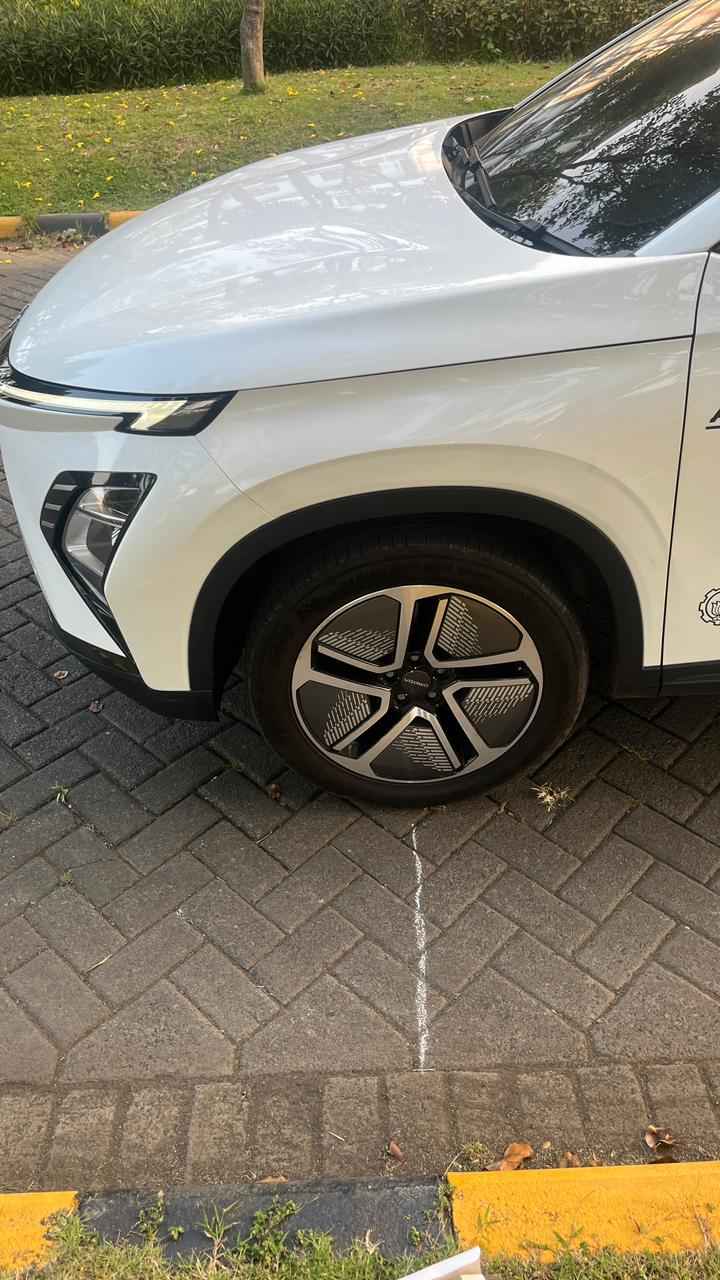
\includegraphics[width=\textwidth]{gambar/start_omoda.jpeg}
        \caption{Omoda E5 ketika memulai proses kalibrasi kecepatan odometri roda.}
        \label{fig:foto_kalibrasi_omoda}
    \end{subfigure}
    \caption{Dokumentasi proses kalibrasi kecepatan odometri roda.}
    \label{fig:kalibrasi_odometri}
\end{figure}

\begin{figure}[H]
    \centering
    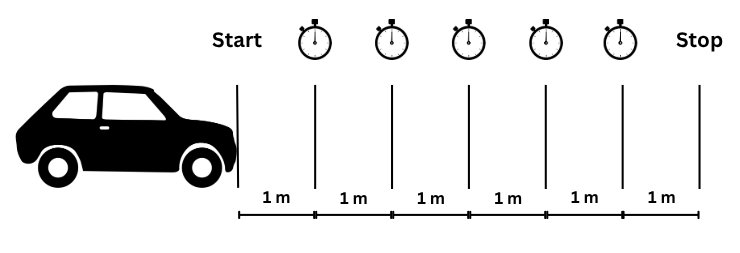
\includegraphics[width=0.8\textwidth]{gambar/kalibrasi_runtime.png}
    \caption{Rencana kalibrasi kecepatan odometri roda dengan mencatat waktu tempuh pada titik acuan.}
    \label{fig:kalibrasi_runtime}
\end{figure}

Varians kecepatan odometri roda diperoleh dengan mengoperasikan kendaraan pada kecepatan konstan 15 km/jam menggunakan fitur \emph{Cruise Control} pada jalan lurus dan datar.
Data kecepatan roda direkam dan dihitung variansnya, menghasilkan nilai ${R}_{odo} = 3{,}25\times10^{-3}$ yang digunakan sebagai matriks kovarians derau pengukuran odometri. Kecepatan roda dikonversi menjadi komponen $v_x$ dan $v_y$ menggunakan orientasi \emph{yaw} yang telah dikoreksi sehingga sesuai dengan kerangka LWA.

\subsubsection{Kalibrasi GPS}

% perlu sitasi NMEA
Tidak seperti IMU dan odometri, akurasi GPS tidak dikalibrasi secara manual.
Modul GPS u-blox ZED-F9P memberikan estimasi akurasi secara langsung dalam format data NMEA (\emph{National Marine Electronics Association}) yang didapat dari data satelit berupa data akurasi posisi horizontal, kecepatan, dan sudut hadap.
Nilai-nilai ini bersifat dinamis dan bergantung pada kondisi sinyal satelit secara \emph{real-time}.
Oleh karena itu, nilai akurasi dari modul digunakan langsung sebagai dasar penentuan matriks kovarians derau pengukuran GPS (${R}_{gps}$) tanpa perlu pengukuran statis terpisah.

Konversi dari koordinat geodetik (\emph{latitude/longitude}) ke kerangka ENU dilakukan dengan menetapkan titik referensi pada posisi GPS pertama saat sistem diinisialisasi. Selisih \emph{latitude} ($\Delta\phi$) dan \emph{longitude} ($\Delta\lambda$) terhadap titik referensi dikonversi ke jarak dalam meter menggunakan panjang satu derajat pada \emph{latitude} $\phi_0$ berdasarkan elipsoid WGS84 \parencite{NIMA2000WGS84}:

\begin{equation}
\Delta E = \Delta\lambda \cdot m_{lon}(\phi_0)
\end{equation}
\begin{equation}
\Delta N = \Delta\phi \cdot m_{lat}(\phi_0)
\end{equation}

dengan $m_{lon}$ dan $m_{lat}$ adalah panjang satu derajat \emph{longitude} dan \emph{latitude} dalam meter yang dihitung menggunakan deret Fourier 3-suku:

\begin{equation}
m_{lon}(\phi_0) = 111412{,}88 \cos\phi_0 - 93{,}50 \cos(3\phi_0) + 0{,}118 \cos(5\phi_0)
\end{equation}
\begin{equation}
m_{lat}(\phi_0) = 111132{,}95 - 559{,}85 \cos(2\phi_0) + 1{,}175 \cos(4\phi_0)
\end{equation}

Data posisi GPS dalam format \emph{latitude/longitude} dikonversi ke kerangka ENU (\emph{East-North-Up}) dengan titik referensi pada posisi GPS pertama diinisialisasi.

\subsection{Kalman Filter \emph{State Vector Position-Velocity}}

Perancangan lokalisasi dengan Kalman Filter menggunakan model \emph{position-velocity} yang mengestimasi posisi dan kecepatan kendaraan dalam kerangka ENU yang terdiri dari vektor \emph{state} $\hat{x} = [x, y, v_x, v_y]^\top$.
Pemilihan model ini didasarkan pada ketersediaan sensor yang memberikan pengukuran posisi (GPS) dan kecepatan (GPS, odometri roda), serta masukan akselerasi dari IMU untuk prediksi model.
Tabel~\ref{tab:kf_params} merangkum parameter utama Kalman Filter yang digunakan.

\begin{table}[H]
\centering
\caption{Parameter Kalman Filter}
\label{tab:kf_params}
\begin{tabular}{l c l}
\hline
\textbf{Parameter} & \textbf{Nilai} & \textbf{Keterangan} \\
\hline
Vektor \emph{state}                    & $[x, y, v_x, v_y]^\top$ & Posisi dan kecepatan dalam ENU \\
Model sistem                           & Kontrol masukan ($u_k$) & Dengan masukan akselerasi IMU \\
Laju pembaruan                         & 100 Hz & Periode 10 ms \\
${R}_{odo}$                     & $3{,}25\times10^{-3}$ & \emph{Measurement noise} odometri \\
${R}_{gps}$                     & Dinamis & Diperbarui berdasarkan data akurasi GPS \\
\hline
\end{tabular}
\end{table}

Siklus Kalman Filter terdiri dari dua tahap utama yang dijalankan secara berulang.
Pada tahap prediksi, akselerasi IMU yang telah dirotasi ke kerangka ENU digunakan untuk memproyeksikan \emph{state} dan kovarians ke langkah waktu berikutnya melalui model sistem kontrol masukan.
Pada tahap koreksi, terdapat dua sumber pengukuran yang digunakan yaitu data GPS dan data odometri roda.
Pengukuran GPS digunakan untuk mengoreksi posisi dan kecepatan \emph{state}, sedangkan odometri roda hanya mengoreksi kecepatan \emph{state}.

Selain koreksi yang sesuai dengan mekanisme standar Kalman Filter, diterapkan juga mekanisme injeksi kecepatan Doppler GPS ketika kendaraan berbelok dengan kecepatan di atas 1,5 m/s dan akurasi kecepatan GPS ($\sigma_{vel}$) di bawah 0,15 m/s yang mengubah \emph{state} kecepatan Kalman Filter.
Hal ini disebabkan oleh roda kendaraan yang mengalami slip saat kendaraan berbelok yang membuat kecepatan roda tidak akurat, sedangkan GPS Doppler mengukur kecepatan relatif terhadap satelit sehingga memberikan estimasi kecepatan yang lebih akurat saat kendaraan bermanuver seperti yang ditunjukkan pada Gambar~\ref{fig:error_odom_belok}.
Fenomena ini dijelaskan oleh \textcite{BouGhosn2024ITSC} di mana kinematik kendaraan dengan \emph{bicycle model} hanya akurat pada percepatan lateral $a_y$ di bawah 0,5 m/s$^2$.

\begin{figure}[H]
    \centering
    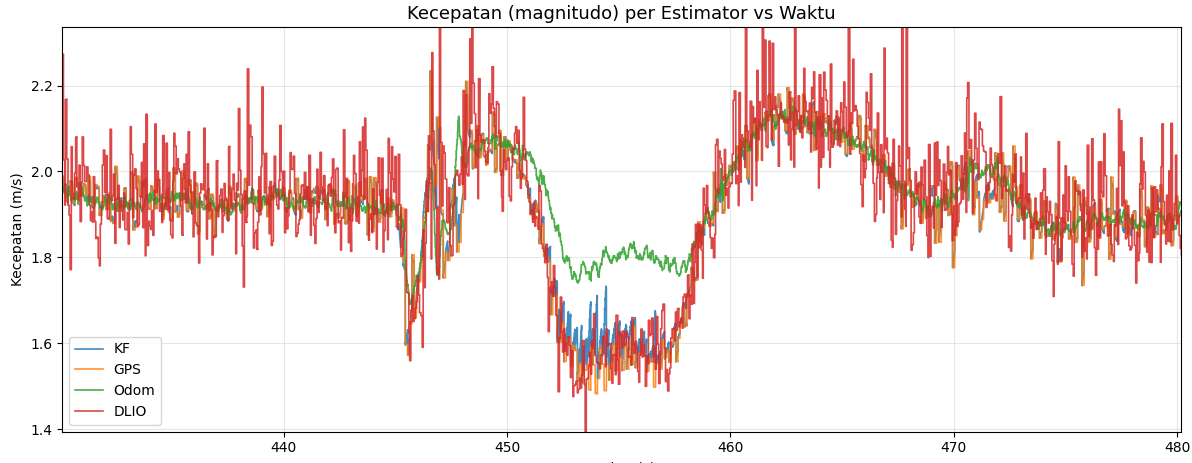
\includegraphics[width=\textwidth]{gambar/error_odom_belok.png}
    \caption{Perbandingan kecepatan Kalman Filter, Odom, GPS, dan DLIO saat kendaraan berbelok.}
    \label{fig:error_odom_belok}
\end{figure}

Koreksi lainnya juga diterapkan ketika kendaraan dalam kondisi diam, di mana posisi GPS yang selalu bergerak (Gambar \ref{fig:error_gps_diam})  meskipun nilai akurasi posisi GPS ($\sigma_{pos}$) di bawah 0,5 m dan akurasi kecepatan GPS ($\sigma_{vel}$) di bawah 0,15 m/s seperti yang ditunjukkan pada Gambar~\ref{fig:error_gps}.
Dalam kondisi ini, posisi GPS tidak akurat sehingga dapat membuat nilai estimasi posisi Kalman Filter menjadi tidak stabil.
Untuk mengatasi masalah ini, diterapkan mekanisme kovarians pengukuran GPS ($R_{gps}$) dinamis berdasarkan parameter akurasi sudut hadap GPS.

\begin{figure}[H]
    \centering
    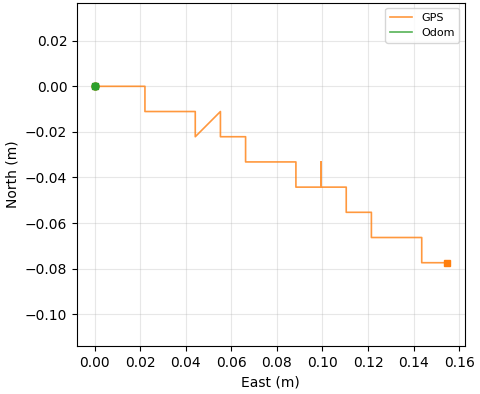
\includegraphics[width=0.8\textwidth]{gambar/error_gps_diam.png}
    \caption{Error posisi GPS saat kendaraan diam.}
    \label{fig:error_gps_diam}
\end{figure}

\begin{figure}[H]
    \centering    
    \begin{subfigure}[b]{0.48\textwidth}
        \centering
        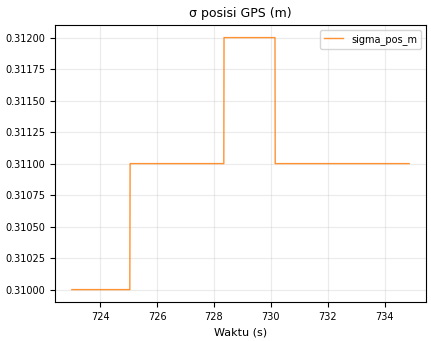
\includegraphics[width=\textwidth]{gambar/error_gps_diam_pos.png}
        \caption{Akurasi posisi GPS saat kendaraan diam.}
        \label{fig:error_gps_diam_pos}
    \end{subfigure}
    \hfill
    \begin{subfigure}[b]{0.48\textwidth}
        \centering
        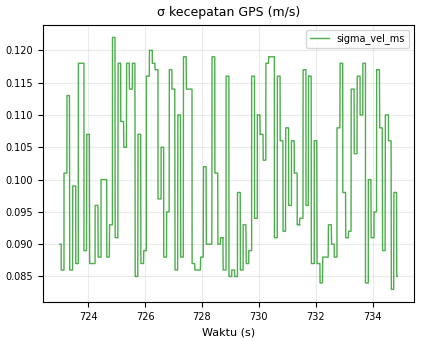
\includegraphics[width=\textwidth]{gambar/error_gps_diam_vel.png}
        \caption{Akurasi kecepatan GPS saat kendaraan diam.}
        \label{fig:error_gps_diam_vel}
    \end{subfigure}
    \caption{Akurasi posisi dan kecepatan GPS saat kendaraan diam}
    \label{fig:error_gps}
\end{figure}


Nilai referensi untuk normalisasi akurasi sudut hadap GPS ditetapkan sebesar 3,0\textdegree.
Pemilihan ini didasarkan pada pengamatan awal di sirkuit terbuka, di mana mayoritas sampel \texttt{head\_acc} berada di bawah 2\textdegree\ dengan median 1,24\textdegree.
Nilai 3,0\textdegree\ yang merupakan 2,4 kali median memberikan margin keamanan yang cukup untuk membedakan kondisi GPS akurat dan tidak akurat tanpa terlalu sensitif terhadap fluktuasi kecil.

Faktor normalisasi $hacc\_norm$ dihitung sebagai:

\begin{equation}
hacc\_norm = \text{clamp}\left(\frac{head\_acc}{3{,}0},\; 1{,}0,\; 10{,}0\right) \times 1{,}5
\label{eq:hacc_norm}
\end{equation}

Nilai $hacc\_norm$ dibatasi pada rentang 1,0 hingga 10,0 untuk mencegah perubahan yang terlalu ekstrem, kemudian dikalikan 1,5 sebagai faktor pengaman.
Kovarians pengukuran posisi GPS ($R_{gps\_pos}$) diubah dengan mengalikan kuadrat $hacc\_norm$ terhadap varians posisi awal:

\begin{equation}
R_{gps\_pos} = \sigma_{pos}^2 \times hacc\_norm^2
\label{eq:r_gps_adaptif}
\end{equation}

Penggunaan kuadrat bertujuan memberikan efek yang lebih signifikan ketika \emph{head\_acc} meningkat, $R_{gps\_pos}$ membesar secara kuadratik sehingga Kalman Gain untuk koreksi GPS menurun drastis dan filter beralih ke prediksi model (IMU + odometri).

\subsection{Skenario Pengujian Lokalisasi}

Pengujian lokalisasi direncanakan dalam empat kategori.
Pertama, validasi terhadap data aktual posisi menggunakan pengukuran fisik dengan pita ukur dan \emph{stopwatch} pada lintasan pendek untuk memperoleh nilai akurasi Kalman Filter.
Kedua, pengujian performa Kalman Filter pada berbagai rute dengan panjang dan karakteristik jalan yang berbeda, menggunakan DLIO sebagai metode pembanding. DLIO dipilih sebagai \emph{baseline} karena akurasinya yang tinggi dan konsisten pada berbagai kondisi lintasan, dengan RMSE hanya 0,0612 m pada segmen dinamis menurut pengujian yang dilakukan oleh \textcite{Chen2023DLIO}.
Ketiga, pengujian ketahanan terhadap degradasi GPS secara alami pada area dengan gedung tinggi untuk mengevaluasi kemampuan sistem mempertahankan estimasi posisi.
Keempat, karakterisasi akurasi sudut hadap pada area terbuka untuk mengetahui hubungan antara kualitas sinyal GPS dan akurasi orientasi IMU.

